\documentclass[letterpaper,11pt]{article}
\usepackage[margin=1in,footskip=0.25in]{geometry}
\setlength{\belowcaptionskip}{-11pt}
\usepackage{multirow}
\usepackage{multicol}
\usepackage{indentfirst}
\usepackage{mathtools} 
\usepackage{amssymb}
\usepackage{mathrsfs}
\usepackage{placeins}
\usepackage{tikz}
\usetikzlibrary{scopes}
\usetikzlibrary{shapes,arrows,decorations.markings,plotmarks}
\usepackage[american]{circuitikz}
\usepackage{bondgraphs}
\usepackage{float}
\usepackage{steinmetz}
\usepackage{graphicx}
\usepackage{textcomp}
\usepackage{gensymb}
\usepackage[utf8]{inputenc}
\usepackage{pgfplots}
\usepackage{booktabs}
\usepackage{ulem}
\usepackage{sectsty}
\usepackage{tcolorbox}
\usepackage{hyperref}
\usepackage{siunitx}
\usepackage{xspace}
\usepackage{advdate}
\pgfplotsset{width=10cm,compat=1.9}

\def\doubleunderline#1{\underline{\underline{#1}}}
\newcounter{MyCounter}
\newcommand{\MATLAB}{\textsc{Matlab}\xspace}

\tikzstyle{block} = [draw, fill=white, rectangle, 
    minimum height=3em, minimum width=6em]
\tikzstyle{sum} = [draw, fill=white, circle, node distance=1cm]
\tikzstyle{input} = [coordinate]
\tikzstyle{output} = [coordinate]
\tikzstyle{pinstyle} = [pin edge={to-,thin,black}]

\title{EAE 130B Block Diagram}
\author{Yihui Li}
\date{\today}

\begin{document}
\begin{figure}[!htb]
    \centering
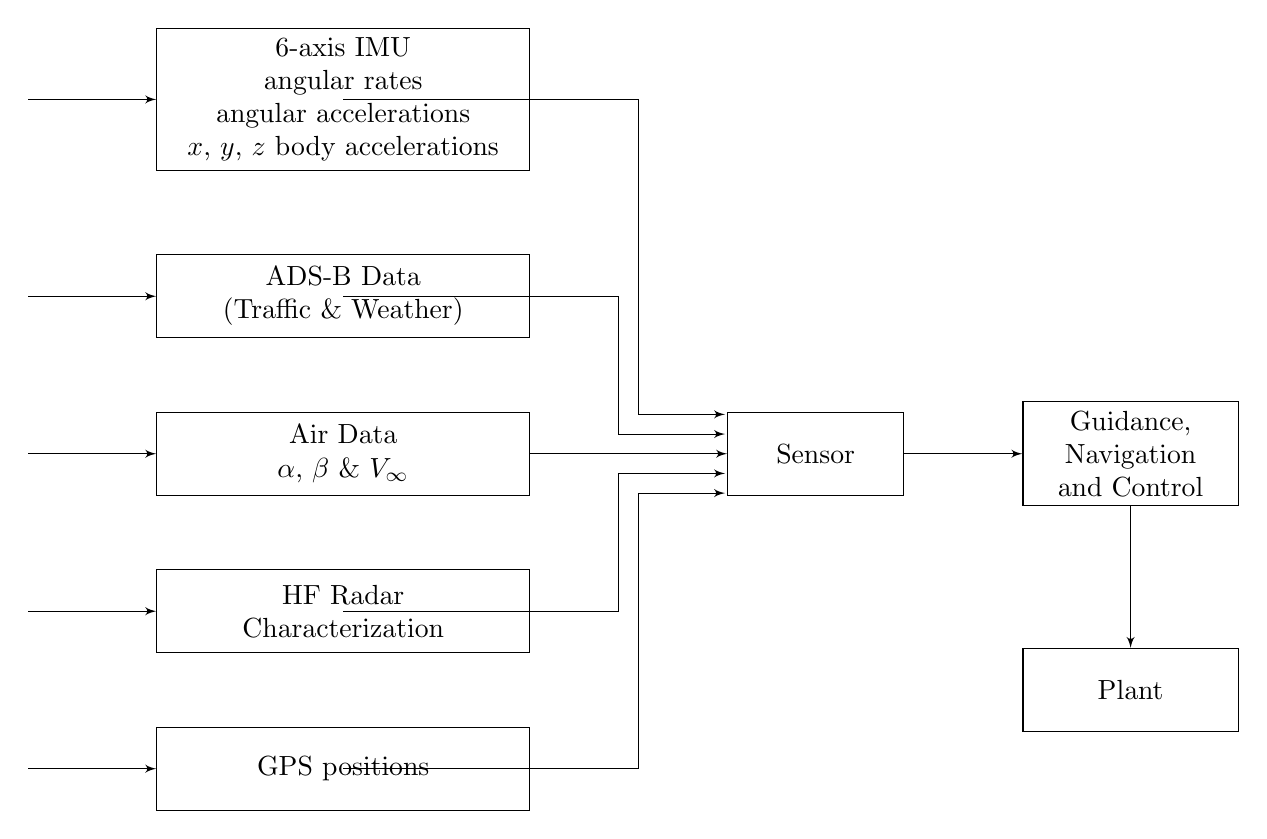
\begin{tikzpicture}[auto, node distance=2cm,>=latex']
% Set-up
	\node [input, name=input3] {};
	\node [input,below of= input3, node distance= 2.0 cm, name=input4] {};
	\node [input,below of= input4, node distance= 2.0 cm, name=input5] {};
	\node [input,above of= input3, node distance= 2.0 cm, name=input2] {};
	\node [input,above of= input2, node distance= 2.5 cm, name=input1] {};
% First column of blocks
	\node [block, right of=input1, node distance= 4.0 cm, align=center, text width= 4.5 cm] (G1) {6-axis IMU\\angular rates\\angular accelerations\\$x$, $y$, $z$ body accelerations};
	\draw [->] (input1) -- node[] {} (G1);
	\node [block, right of=input2, node distance= 4.0 cm, align=center, text width = 4.5 cm] (G2) {ADS-B Data\\(Traffic \& Weather)};
	\draw [->] (input2) -- node[] {} (G2);
	\node [block, right of=input3, node distance= 4.0 cm, align=center, text width = 4.5 cm] (G3) {Air Data\\$\alpha$, $\beta$ \& $V_\infty$};
	\draw [->] (input3) -- node[] {} (G3);	
	\node [block, right of=input4, node distance= 4.0 cm, align=center, text width = 4.5 cm] (G4) {HF Radar\\Characterization};
	\draw [->] (input4) -- node[] {} (G4);
	\node [block, right of=input5, node distance= 4.0 cm, align=center, text width = 4.5 cm] (G5) {GPS positions};
	\draw [->] (input5) -- node[] {} (G5);
% Second column of block
	\node [block, right of=G3, node distance= 6.0 cm, align=center, text width = 2.0 cm] (H1) {Sensor};
% Arrows between first and second column
%%%%  	\foreach \X in {1,2,4,5} can be used here, but it is removed for others' convenience
	%% G1
		\node [input, right of = G1, node distance = 3.75 cm, name=aref1] {};
		\node [input, above of = H1, node distance = 0.5 cm, name=bref1] {};
		\node[input, left of = bref1, node distance = 1.15 cm, name=cref1] {};
		\draw [-] (G1) |- (aref1);
		\draw [->] (aref1) |- (cref1);
	%% G2
		\node [input, right of = G2, node distance = 3.50 cm, name=aref2] {};
		\node [input, above of = H1, node distance = 0.25 cm, name=bref2] {};
		\node[input, left of = bref2, node distance = 1.15 cm, name=cref2] {};
		\draw [-] (G2) |- (aref2);
		\draw [->] (aref2) |- (cref2);
	%% G3
	\draw [->] (G3) -- node {} (H1);
	%% G4
		\node [input, right of = G4, node distance = 3.50 cm, name=aref4] {};
		\node [input, below of = H1, node distance = 0.25 cm, name=bref4] {};
		\node[input, left of = bref4, node distance = 1.15 cm, name=cref4] {};
		\draw [-] (G4) |- (aref4);
		\draw [->] (aref4) |- (cref4);
	%% G5
		\node [input, right of = G5, node distance = 3.75 cm, name=aref5] {};
		\node [input, below of = H1, node distance = 0.50 cm, name=bref5] {};
		\node[input, left of = bref5, node distance = 1.15 cm, name=cref5] {};
		\draw [-] (G5) |- (aref5);
		\draw [->] (aref5) |- (cref5);
% Third column of block
	\node [block, right of=H1, node distance= 4.0 cm, align=center, text width = 2.5 cm] (I1) {Guidance, Navigation and Control};
	\draw [->] (H1) -- node[] {} (I1);
% Last block
	\node [block, below of=I1, node distance= 3.0 cm, align=center, text width = 2.5 cm] (J1) {Plant};
	\draw [->] (I1) -- node[] {} (J1);
\end{tikzpicture}
\caption{Block diagram.}
\label{fig:blockdiagram}
\end{figure}
\end{document}